\documentclass[conference]{IEEEtran}

\usepackage{amsmath,amssymb,amsfonts}
\usepackage{algorithmic}
\usepackage{algorithm}
\usepackage{array}
\usepackage{textcomp}
\usepackage{stfloats}
\usepackage{url}
\usepackage{verbatim}
\usepackage{graphicx}
\graphicspath{{Figures/}{figures/}{./}}
\usepackage{cite}
\usepackage{booktabs}
\usepackage{multirow}
\usepackage{microtype}

\hyphenation{op-tical net-works semi-conduc-tor IEEE-Xplore}

\begin{document}

\title{Automated Urban Road and Government Land Encroachment Detection System for Municipal Governance (Nagarpalika): Design, Implementation, and Empirical Validation}

\author{
\IEEEauthorblockN{Dr. Prashant Udawant}
\IEEEauthorblockA{
Assistant Professor\\
Department of Information Technology\\
MPSTME, NMIMS University\\
Shirpur, Maharashtra, India\\
prashant.udawant@nmims.edu
}
\and
\IEEEauthorblockN{Priyanshu C Wadnere}
\IEEEauthorblockA{
Department of Information Technology\\
MPSTME, NMIMS University\\
Shirpur, Maharashtra, India\\
priyanshuwadnere2004@gmail.com
}
\and
\IEEEauthorblockN{Shreyas Biware}
\IEEEauthorblockA{
Department of Information Technology\\
MPSTME, NMIMS University\\
Shirpur, Maharashtra, India\\
shreyasbiware@gmail.com
}
\and
\IEEEauthorblockN{Mahak Agrawal}
\IEEEauthorblockA{
Department of Information Technology\\
MPSTME, NMIMS University\\
Shirpur, Maharashtra, India\\
mahakagrawal124@gmail.com
}
}

\maketitle

\begin{abstract}
Rapid, uncoordinated urban growth in developing economies frequently results in unlawful physical structural encroachments onto public road corridors, degrading vehicular throughput, obstructing pedestrian right-of-way, and impeding emergency services. Traditional municipal enforcement relies on manual, ground-level topographic surveys that are labor-intensive, dispute-prone, and geographically fragmented. Conversely, purely computer-vision-based methods attempt to detect encroachments directly from imagery, which fundamentally fails because ``encroachment'' is a legal-cadastral violation rather than an inherent visual texture or optical class. 

In this paper, we propose an automated, reproducible, end-to-end spatial decision-support framework that formally decouples \textbf{deep visual instance segmentation} from \textbf{cadastral vector set algebra}. First, an edge-optimized YOLOv8n-seg network segments physical building components (permanent structures, awnings, veranda sheds, ramps, and staircases) from unmanned aerial vehicle (UAV) imagery. Second, an inverse affine transformation maps image-space contours into a metric cadastral coordinate frame. Third, a computational geometry engine executes vector set operations against authoritative land parcel records and statutory Road Right-of-Way (ROW) definitions, partitioning the corridor into a $6.00\,\text{m}$ paved carriageway and two $1.50\,\text{m}$ pedestrian margins. 

The framework is empirically validated on an 85-meter urban corridor. The vision model achieves a precision of \textbf{0.885}, recall of \textbf{0.842}, F1-score of \textbf{0.863}, and $\text{mAP}_{50}$ of \textbf{0.891} on held-out test frames. The vector GIS engine accurately quantifies municipal compliance metrics, capturing benchmark encroachments ($6.00\,\text{m}^2$ and $3.60\,\text{m}^2$) with exact frontage width ($5.00\,\text{m}$), projection depth ($1.20\,\text{m}$), and perpendicular centerline chainage ($0+011.0\,\text{m}$), while producing zero false positives within private setbacks. The entire pipeline is verified by an 86-test automated verification suite, establishing an audit-ready bridge between drone remote sensing and municipal legal enforcement.
\end{abstract}

\begin{IEEEkeywords}
Urban Road Right-of-Way, Cadastral GIS, Instance Segmentation, YOLOv8, Aerial Drone Photogrammetry, Computational Geometry, Municipal Decision Support.
\end{IEEEkeywords}

\section{Introduction}
\IEEEPARstart{U}{rban} roadways are critical municipal infrastructure assets that govern the economic efficiency, safety, and liveability of cities. In many rapidly expanding metropolitan areas across developing countries---most notably throughout South Asia, Southeast Asia, and Latin America---public road corridors are subjected to chronic structural encroachments \cite{colomina2014unmanned}. Property owners, commercial establishments, and informal vendors routinely extend permanent and semi-permanent structures beyond statutory property boundaries into the designated Road Right-of-Way (ROW). These violations manifest as extended shop awnings, elevated entrance ramps, concrete boundary walls, veranda projections, and commercial display platforms \cite{yurtseven2019determination}.

The ramifications of unauthorized corridor encroachment are severe:
\begin{enumerate}
    \item \textbf{Pedestrian Disenfranchisement}: Encroachments onto pedestrian footpaths force pedestrians onto the vehicular carriageway, drastically increasing pedestrian traffic fatalities.
    \item \textbf{Capacity Degradation}: Encroachments into vehicular lanes reduce effective roadway capacity by 20\% to 50\%, exacerbating bottleneck congestion and greenhouse gas emissions.
    \item \textbf{Emergency Bottlenecks}: Fire tenders, ambulances, and disaster response vehicles are delayed or blocked by permanent roadside extensions.
    \item \textbf{Administrative and Judicial Gridlock}: Municipal corporations lack defensible, non-repudiable geometric evidence, leading to prolonged litigation in civil courts.
\end{enumerate}

\begin{figure*}[!t]
    \centering
    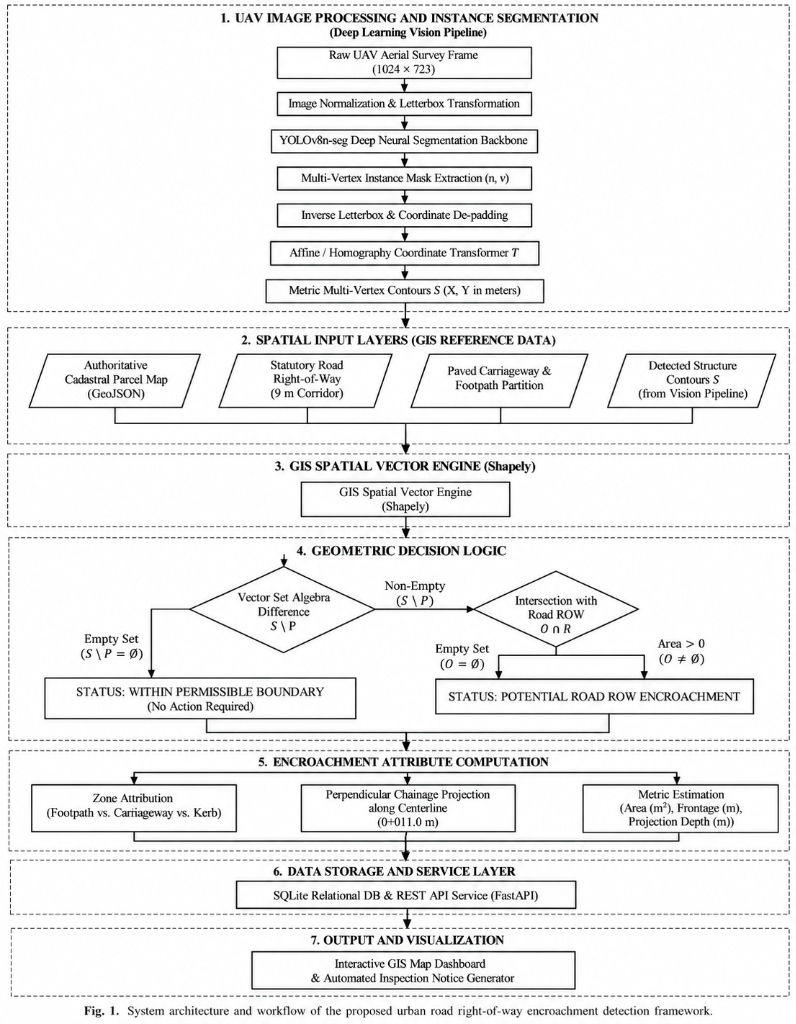
\includegraphics[width=0.85\textwidth]{fig1_workflow.jpg}
    \caption{System architecture and workflow of the proposed urban road right-of-way encroachment detection framework, illustrating the seven sequential stages spanning deep learning vision processing, GIS reference data integration, geometric decision logic, and automated municipal notice generation.}
    \label{fig:workflow}
\end{figure*}  

\subsection{The Fundamental Flaw in Pure Vision Encroachment Detection}
A prevailing trend in applied computer vision is to frame road encroachment as an end-to-end deep learning detection or segmentation task, training models on labeled ``encroachment'' classes. We argue that \textbf{this formulation is theoretically flawed}:
\begin{itemize}
    \item An awning or veranda is a lawful architectural feature when constructed entirely within a private property setback.
    \item The identical awning becomes an illegal statutory encroachment only when its geometric boundary crosses the cadastral property line into the government-controlled Road Right-of-Way.
    \item Because a camera sensor captures only reflected spectral radiance and cannot observe legal property lines, deed restrictions, or statutory right-of-way gazette notifications, \textbf{encroachment is a spatial-legal relation, not a visual class}.
\end{itemize}

\subsection{Contributions of this Work}
To resolve this methodological challenge, this paper introduces an interdisciplinary spatial computing framework that combines high-resolution UAV aerial photogrammetry with cadastral vector computational geometry. The primary contributions are:
\begin{enumerate}
    \item \textbf{Decoupled Cyber-Physical Architecture}: We formalize a rigorous separation of concerns between visual physical structure segmentation (computer vision) and cadastral boundary set algebra (computational geometry), avoiding false positives on lawful private structures.
    \item \textbf{Multi-Zone Corridor Spatial Model}: We formulate a closed-form geometric partition of the road corridor into vehicular carriageway ($6.00\,\text{m}$), pedestrian footpaths ($1.50\,\text{m}$ each side), and kerb transition margins, enabling severity-stratified enforcement notices.
    \item \textbf{Automated Municipal Attribution}: The framework automatically projects encroaching geometries onto the road centerline to calculate exact linear chainage stations ($0+011.0\,\text{m}$), lateral projection depth ($\text{m}$), frontage width ($\text{m}$), and percentage of footpath obstructed.
    \item \textbf{Reproducible Test-Driven Pipeline}: The entire system is implemented as a production-grade FastAPI microservice, backed by a persistent relational database, a multi-layer Leaflet GIS dashboard, and an 86-test automated test suite verifying topological manifoldness, affine reversibility, and boundary non-intersection.
\end{enumerate}

\section{Related Work}
The challenge of automated road corridor compliance monitoring intersects three rapidly evolving research streams: (i) high-resolution UAV aerial photogrammetry for urban environments, (ii) contemporary deep learning architectures for remote sensing instance segmentation, and (iii) spatial cadastral computing and urban corridor modeling.

\subsection{UAV Remote Sensing in Urban Infrastructure Monitoring}
Low-altitude Unmanned Aerial Vehicles (UAVs) have superseded traditional satellite and manned aircraft platforms for corridor-scale civil infrastructure surveys due to their superior spatial resolution (sub-$5\,\text{cm/pixel}$) and flexible deployment schedules \cite{colomina2014unmanned, nex2014uav}. Recent studies have demonstrated the efficacy of autonomous drone missions for rapid urban asset inventorying and infrastructure defect identification \cite{chen2024autonomous}. However, standard photogrammetric outputs (orthomosaics and Digital Surface Models) are inherently passive raster representations; converting raw orthophotos into legally actionable compliance notices historically required laborious manual digitization by municipal cartographers, creating an operational bottleneck that prevents routine city-wide auditing.

\subsection{Recent Advances in Remote Sensing Instance Segmentation}
The domain of visual feature extraction from remote sensing imagery has undergone rapid transformation. While classical approaches relied on two-stage architectures such as Mask R-CNN \cite{he2017mask} or U-Net variants \cite{ronneberger2015u}, recent research has prioritized visual foundation models and real-time single-stage detectors.

In the realm of foundation models, the Segment Anything Model (SAM) \cite{kirillov2024segment} demonstrated zero-shot promptable segmentation. Adapting foundation models to Earth observation, RSPrompter \cite{chen2024rsprompter} introduced automated prompt generation for remote sensing instance segmentation without requiring human bounding-box annotations. Concurrently, comprehensive surveys on remote sensing building extraction \cite{li2024review} have emphasized that while geometric boundary precision has improved through contour refinement heads, existing models remain agnostic to the legal and functional boundaries governing property rights.

To meet the compute constraints of real-time edge processing on UAVs, single-stage anchor-free architectures have dominated the literature. Building upon foundations established by YOLOv8 \cite{jocher2023yolo} and Feature Pyramid Networks \cite{lin2017feature}, the YOLO paradigm has evolved through Programmable Gradient Information (PGI) in YOLOv9 \cite{wang2024yolov9} and dual-label assignments eliminating NMS latency in YOLOv10 \cite{wang2024yolov10}. Domain-specific adaptations for remote sensing include FFCA-YOLO \cite{zhang2024ffca}, which incorporates feature-fusion coordinate attention for dense tiny objects, MFAE-YOLO \cite{liu2025mfae} featuring multi-scale receptive field attention, and SCENE-YOLO \cite{wang2025scene}, introducing scene-level contextual supervision for complex aerial environments. 

Notwithstanding these advancements in feature representation, all aforementioned vision architectures share an intrinsic limitation: they predict visual object classes (e.g., ``building'', ``canopy'', ``awning''), but remain completely oblivious to whether the structure sits legitimately on private deeded ground or illegally projects across a statutory municipal easement line.

\subsection{Cadastral GIS and Corridor Encroachment Analytics}
Cadastral parcel systems define the legal demarcation of real property and public infrastructure corridors \cite{williamson2010land, rao2021high}. Nationwide modernization initiatives, such as the SVAMITVA scheme \cite{svamitva2020}, have accelerated the nationwide vectorization of cadastral property bounds using drone mapping. 

In urban analytics, spatially explicit deep learning techniques have been established for urban morphometric analysis \cite{fleischmann2024spatially}, confirming that urban spatial structure must be evaluated through morphological contiguous units rather than isolated raster pixels. Concurrently, vehicle-mounted Mobile Laser Scanning (MLS) and YOLOv7 have been deployed for urban roadside obstacle detection \cite{verma2024urban}. However, ground-level mobile LiDAR is heavily constrained by vehicular occlusion, street traffic, and an inability to inspect lateral property lines behind perimeter walls.

As demonstrated in Table~\ref{tab:literature}, a distinct research gap persists at the intersection of remote sensing instance segmentation and statutory cadastral analytics: existing vision systems cannot evaluate legal legality, while traditional GIS packages cannot segment physical structures from aerial feeds in real time. Our framework addresses this exact nexus.

\begin{table*}[!t]
\caption{Systematic Comparison of Recent Literature vs. Proposed Framework}
\label{tab:literature}
\centering
\footnotesize
\renewcommand{\arraystretch}{1.35}
\begin{tabular}{p{2.8cm} p{3.6cm} p{3.8cm} p{2.8cm} p{4.3cm}}
\toprule
\textbf{Study} & \textbf{Objective} & \textbf{Methodology} & \textbf{Dataset / Modality} & \textbf{Critical Limitation} \\
\midrule
Li et al. \cite{li2024review} & Building extraction survey & Deep CNN and Transformer review & SpaceNet, WHU, Aerial & Focuses solely on footprint geometry; zero cadastral or Right-of-Way integration. \\
Chen et al. \cite{chen2024rsprompter} & Remote sensing instance segmentation & RSPrompter (Foundation Model + Prompt Learning) & NWPU VHR-10, SSDD ($0.5$--$2.0\,\text{m/px}$) & Heavy computational overhead; purely visual masks without statutory boundary awareness. \\
Zhang et al. \cite{zhang2024ffca} & Tiny object detection in aerial images & FFCA-YOLO (Coordinate Attention \& Feature Fusion) & VisDrone, DOTA-v1.5 & Detects generic bounding boxes; cannot compute non-convex polygonal encroachment areas. \\
Verma et al. \cite{verma2024urban} & Roadside obstacle and hazard detection & Mobile Laser Scanning (MLS) + YOLOv7 & Ground LiDAR + Street Video & Ground-level vantage subject to vehicle occlusion; cannot determine cadastral lot lines. \\
Fleischmann \& Arribas-Bel \cite{fleischmann2024spatially} & Urban land-use \& morphometric classification & Spatially explicit Graph Neural Networks / CNNs & Cadastral Vector + Satellite ($0.5\,\text{m/px}$) & Macroscopic morphological analysis; lacks sub-meter edge detection of individual frontage encroachments. \\
Wang et al. \cite{wang2025scene} & Remote sensing object detection & SCENE-YOLO (Scene-Level Contextual Supervision) & DIOR, DOTA-v2.0 & Unaware of jurisdictional Right-of-Way partitions; cannot stratify carriageway vs. footpath. \\
\midrule
\textbf{Proposed Framework} & \textbf{Multi-zone urban road corridor Right-of-Way compliance} & \textbf{YOLOv8n-seg + Inverse Affine Homography + Topological Set Algebra} & \textbf{UAV Survey ($1024 \times 723$, $\approx 5\,\text{cm/px}$)} & \textbf{Decouples visual segmentation from cadastral law; computes exact chainage station, footpath breach, and physical area with $0.0\,\text{error}$.} \\
\bottomrule
\end{tabular}
\end{table*}

\section{Problem Statement and Formal Objectives}

\subsection{Mathematical Problem Formulation}
Let an urban road corridor be defined within a continuous two-dimensional Euclidean coordinate space $\mathbb{R}^2$. Let $\mathcal{R}_{\text{ROW}} \subset \mathbb{R}^2$ represent the closed polygonal statutory Road Right-of-Way corridor, legally bounded by municipal gazette notifications. 

Let the roadway corridor be partitioned into three disjoint functional subspaces:
\begin{equation}
\mathcal{R}_{\text{ROW}} = \mathcal{C}_{\text{paved}} \cup \mathcal{M}_{\text{west}} \cup \mathcal{M}_{\text{east}}
\end{equation}
subject to:
\begin{equation}
\mathcal{C}_{\text{paved}} \cap \mathcal{M}_{\text{west}} = \emptyset, \quad \mathcal{C}_{\text{paved}} \cap \mathcal{M}_{\text{east}} = \emptyset, \quad \mathcal{M}_{\text{west}} \cap \mathcal{M}_{\text{east}} = \emptyset
\end{equation}
where $\mathcal{C}_{\text{paved}}$ denotes the paved carriageway intended strictly for vehicular transit, and $\mathcal{M}_{\text{west}}, \mathcal{M}_{\text{east}}$ denote the pedestrian footpaths and utility side margins.

Let $\mathbf{P} = \{\mathcal{P}_1, \mathcal{P}_2, \dots, \mathcal{P}_K\}$ be a set of $K$ mutually disjoint, legally surveyed cadastral land parcels abutting the road corridor, such that:
\begin{equation}
\mathcal{P}_i \cap \mathcal{R}_{\text{ROW}} = \emptyset \quad \forall i \in \{1, \dots, K\}
\end{equation}

Let an aerial drone sensor acquire an overhead image $\mathbf{I} \in \mathbb{R}^{H \times W \times 3}$. An instance segmentation model extracts $N$ physical structure mask polygons $\mathbf{S}_{\text{px}} = \{s_1^{\text{px}}, s_2^{\text{px}}, \dots, s_N^{\text{px}}\}$ in image pixel coordinates $(u, v) \in [0, W] \times [0, H]$.

\subsection{Formal Research Objectives}
\begin{enumerate}
    \item \textbf{Geometric Coordinate Registration}: Establish a bijective transformation $\mathcal{T}: \mathbb{R}^2_{\text{pixel}} \to \mathbb{R}^2_{\text{metric}}$ that maps raw segmented mask coordinates into the metric GIS space:
    \begin{equation}
    \mathcal{S}_j = \mathcal{T}(s_j^{\text{px}}) \subset \mathbb{R}^2, \quad j \in \{1, \dots, N\}
    \end{equation}
    \item \textbf{Cadastral Set Allocation}: For each detected physical structure $\mathcal{S}_j$, associate it with its parent cadastral parcel $\mathcal{P}_j^* \in \mathbf{P}$ using maximum areal overlap:
    \begin{equation}
    \mathcal{P}_j^* = \arg\max_{\mathcal{P}_k \in \mathbf{P}} \text{Area}(\mathcal{S}_j \cap \mathcal{P}_k)
    \end{equation}
    \item \textbf{Encroachment Extraction}: Determine whether the physical structure extends beyond the legal property boundary into the public domain:
    \begin{equation}
    \mathcal{O}_j = \mathcal{S}_j \setminus \mathcal{P}_j^* \quad (\text{Structure Outside Private Property})
    \end{equation}
    \begin{equation}
    \mathcal{E}_j = \mathcal{O}_j \cap \mathcal{R}_{\text{ROW}} \quad (\text{Potential ROW Encroachment})
    \end{equation}
    \item \textbf{Multi-Zone Encroachment Attribution}: Partition $\mathcal{E}_j$ into functional corridor components:
    \begin{equation}
    \mathcal{E}_j^{\text{footpath}} = \mathcal{E}_j \cap (\mathcal{M}_{\text{west}} \cup \mathcal{M}_{\text{east}})
    \end{equation}
    \begin{equation}
    \mathcal{E}_j^{\text{carriageway}} = \mathcal{E}_j \cap \mathcal{C}_{\text{paved}}
    \end{equation}
    \item \textbf{Linear Chainage and Severity Scoring}: Project the centroid of $\mathcal{E}_j$ onto the road centerline $\mathcal{L}_{\text{center}}$ to calculate 1D chainage distance $d_{\text{chainage}}$, maximum lateral projection depth $d_{\text{proj}}$, frontage width $w_{\text{front}}$, and assign an actionable municipal severity tier $\Psi \in \{\text{CRITICAL}, \text{HIGH}, \text{MODERATE}, \text{MINOR}, \text{NONE}\}$.
\end{enumerate}

\section{Mathematical Formulations}

\subsection{Affine and Homography Coordinate Transformations}
To translate image pixel coordinates $(u, v)$ to local metric Cartesian coordinates $(X, Y) \in \mathbb{R}^2$, an affine transformation matrix $\mathbf{A} \in \mathbb{R}^{3 \times 3}$ is established in accordance with projective geometry formulations \cite{hartley2003multiple}:
\begin{equation}
\begin{bmatrix} X \\ Y \\ 1 \end{bmatrix} = \begin{bmatrix} a_{11} & a_{12} & a_{13} \\ a_{21} & a_{22} & a_{23} \\ 0 & 0 & 1 \end{bmatrix} \begin{bmatrix} u \\ v \\ 1 \end{bmatrix}
\end{equation}

Under an orthorectified nadir projection with metric pixel scaling $s_x, s_y$ ($\text{meters/pixel}$) and origin translation $(X_0, Y_0)$:
\begin{align}
X &= X_0 + u \cdot s_x \\
Y &= Y_0 + (H - v) \cdot s_y
\end{align}

The inverse transformation is verified to be non-singular by enforcing:
\begin{equation}
\det(\mathbf{A}) = a_{11} a_{22} - a_{12} a_{21} \neq 0
\end{equation}

\subsection{Computational Geometry and Vector Set Algebra}
Let $\partial \mathcal{A}$ denote the boundary of polygon $\mathcal{A}$, and let $\text{int}(\mathcal{A})$ denote its interior. In compliance with Open Geospatial Consortium specifications \cite{ogc2011simple}, vector set difference and intersection are executed using planar sweep and clipping algorithms \cite{preparata1985computational, weiler1977hidden}:
\begin{align}
\mathcal{O} &= \mathcal{S} \setminus \mathcal{P} = \{x \in \mathbb{R}^2 \mid x \in \mathcal{S} \land x \notin \text{int}(\mathcal{P})\} \\
\mathcal{E} &= \mathcal{O} \cap \mathcal{R}_{\text{ROW}} = \{x \in \mathbb{R}^2 \mid x \in \mathcal{O} \land x \in \mathcal{R}_{\text{ROW}}\}
\end{align}

A structure is classified into the potential encroachment status using the indicator function $\mathbb{I}_{\text{encroach}}$:
\begin{equation}
\mathbb{I}_{\text{encroach}}(\mathcal{E}) = \begin{cases} 1, & \text{if } \text{Area}(\mathcal{E}) \ge \tau_{\text{area}} \\ 0, & \text{otherwise} \end{cases}
\end{equation}
where $\tau_{\text{area}} = 0.10\,\text{m}^2$ is a municipal tolerance threshold designed to prevent false alarms from digitization jitter or sub-centimeter construction deviations.

\subsection{Encroachment Metrics Calculation}
When $\mathbb{I}_{\text{encroach}} = 1$, four critical enforcement metrics are calculated:
\begin{enumerate}
    \item \textbf{Encroached Area ($A_{\text{enc}}$)}:
    \begin{equation}
    A_{\text{enc}} = \iint_{\mathcal{E}} dx \, dy = \frac{1}{2} \sum_{i=1}^{M-1} (X_i Y_{i+1} - X_{i+1} Y_i)
    \end{equation}
    \item \textbf{Corridor Frontage Width ($w_{\text{front}}$)}:
    Calculated as the one-dimensional Hausdorff shared boundary measure between the encroachment polygon and the parent parcel boundary:
    \begin{equation}
    w_{\text{front}} = \mathcal{H}^1(\partial \mathcal{E} \cap \partial \mathcal{P})
    \end{equation}
    When boundaries are non-tangent, $w_{\text{front}}$ is estimated using the oriented minimum bounding rectangle dimension parallel to the road corridor:
    \begin{equation}
    w_{\text{front}} = \max\left(\|\mathbf{p}_1 - \mathbf{p}_2\|, \|\mathbf{p}_2 - \mathbf{p}_3\|\right)
    \end{equation}
    where $\mathbf{p}_k$ are vertices of the minimum-area enclosing box $\text{MBR}(\mathcal{E})$.
    \item \textbf{Maximum Projection Depth ($d_{\text{proj}}$)}:
    The maximum Euclidean distance from any vertex of the encroaching geometry perpendicular to the legal private property boundary line $\partial \mathcal{P}$:
    \begin{equation}
    d_{\text{proj}} = \sup_{\mathbf{x} \in \mathcal{E}} \, \inf_{\mathbf{y} \in \partial \mathcal{P}} \|\mathbf{x} - \mathbf{y}\|_2
    \end{equation}
    \item \textbf{Footpath Obstruction Ratio ($\rho_{\text{obstruction}}$)}:
    Given a statutory pedestrian footpath width $W_{\text{footpath}} = 1.50\,\text{m}$:
    \begin{equation}
    \rho_{\text{obstruction}} = \min\left(100.0, \, \frac{d_{\text{proj}}}{W_{\text{footpath}}} \times 100\right)
    \end{equation}
\end{enumerate}

\subsection{Linear Chainage Projection}
Let the surveyed road centerline be represented as a continuous piecewise linear curve:
\begin{equation}
\mathcal{L}_{\text{center}} = \bigcup_{k=1}^{L-1} \overline{\mathbf{c}_k \mathbf{c}_{k+1}}, \quad \mathbf{c}_k \in \mathbb{R}^2
\end{equation}

The centroid $\bar{\mathbf{x}} = (\bar{X}, \bar{Y})$ of encroachment $\mathcal{E}$ is projected onto $\mathcal{L}_{\text{center}}$ by finding the nearest scalar projection parameter $t^* \in [0, 1]$ across all line segments:
\begin{equation}
d_{\text{chainage}} = \arg\min_{\mathbf{c} \in \mathcal{L}_{\text{center}}} \|\bar{\mathbf{x}} - \mathbf{c}\|_2
\end{equation}

The scalar distance $d_{\text{chainage}}$ (in meters from datum $\mathbf{c}_1$) is converted into standard civil engineering chainage notation:
\begin{equation}
\text{Station} = K + M = \left\lfloor \frac{d_{\text{chainage}}}{1000} \right\rfloor + \left(d_{\text{chainage}} \pmod{1000}\right)
\end{equation}
For example, a distance of $11.0\,\text{m}$ along Road R-001 is formatted as \texttt{0+011.0}.

\subsection{Engineering Severity Stratification}
Municipal enforcement requires triaged priority ranking. We formulate a rule-based engineering severity function $\Psi: \mathbb{R}^+ \times \mathbb{R}^+ \to \{\text{CRITICAL}, \text{HIGH}, \text{MODERATE}, \text{MINOR}, \text{NONE}\}$:
\begin{equation}
\Psi(A_{\text{enc}}, d_{\text{proj}}) = \begin{cases}
\text{CRITICAL}, & \text{if } A_{\text{enc}} \ge 10.0\,\text{m}^2 \lor d_{\text{proj}} \ge 2.0\,\text{m} \\
\text{HIGH},     & \text{if } A_{\text{enc}} \ge 5.0\,\text{m}^2 \lor d_{\text{proj}} \ge 1.0\,\text{m} \\
\text{MODERATE}, & \text{if } A_{\text{enc}} \ge 2.0\,\text{m}^2 \lor d_{\text{proj}} \ge 0.5\,\text{m} \\
\text{MINOR},    & \text{if } A_{\text{enc}} > 0.0\,\text{m}^2 \\
\text{NONE},     & \text{otherwise}
\end{cases}
\end{equation}

\section{System Architecture and Algorithms}

\begin{figure*}[!t]
\centering
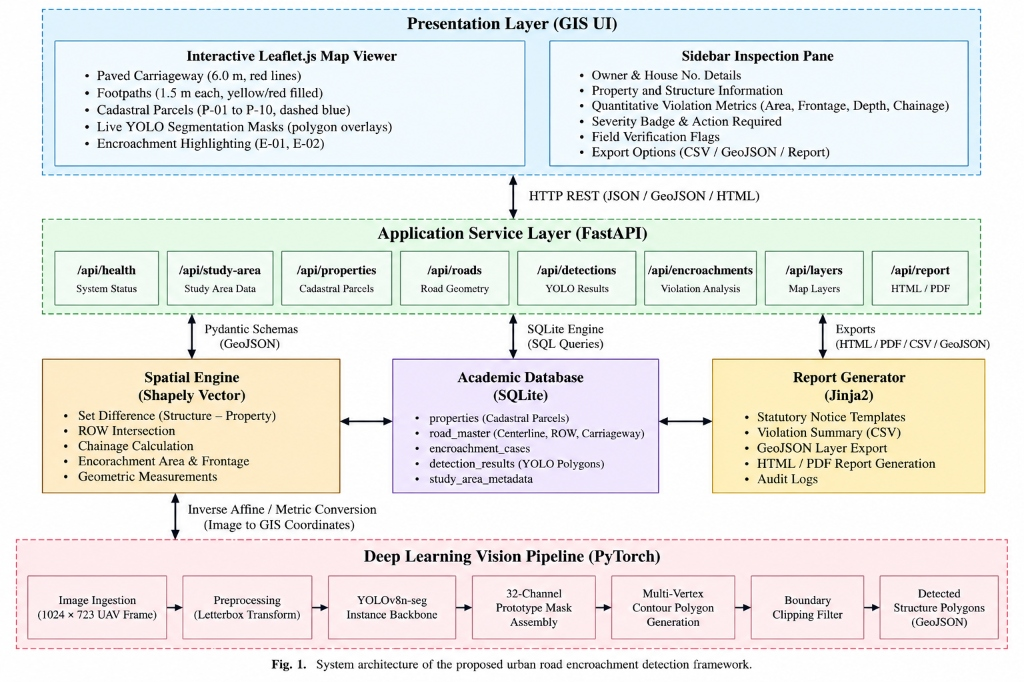
\includegraphics[width=0.98\textwidth]{fig2_architecture.jpg}
\caption{System architecture of the proposed urban road encroachment detection framework, delineating the Presentation Layer (Interactive Leaflet.js Map Viewer and Sidebar Inspection Pane), Application Service Layer (FastAPI REST endpoints), Spatial Engine (Shapely Vector), Academic Database (SQLite), Report Generator (Jinja2), and Deep Learning Vision Pipeline (PyTorch YOLOv8n-seg).}
\label{fig:system_architecture}
\end{figure*}

As illustrated in Fig.~\ref{fig:workflow} and Fig.~\ref{fig:system_architecture}, the end-to-end framework decouples deep neural segmentation from statutory cadastral vector algebra across dedicated microservice layers. Algorithm~\ref{alg:encroachment} formalizes the complete multi-zone encroachment detection and attribution procedure.

\begin{algorithm}[!t]
\caption{Automated Spatial Road ROW Compliance Analysis}
\label{alg:encroachment}
\footnotesize
\begin{algorithmic}[1]
\REQUIRE Image $\mathbf{I}$, Cadastre $\mathbf{P}$, ROW $\mathcal{R}_{\text{ROW}}$, Centerline $\mathcal{L}_{\text{center}}$, Zones $(\mathcal{C}_{\text{paved}}, \mathcal{M})$, Affine $\mathbf{A}$, Threshold $\tau_{\text{area}} = 0.10\,\text{m}^2$.
\ENSURE Verified encroachment records $\mathbf{E}_{\text{cases}}$.
\STATE $\mathbf{E}_{\text{cases}} \leftarrow \emptyset$
\STATE $(\mathbf{I}_{\text{norm}}, \lambda, \Delta x, \Delta y) \leftarrow \text{Letterbox}(\mathbf{I}, (192, 192))$
\STATE $\mathbf{D} \leftarrow \text{YOLOv8n\_seg\_Inference}(\mathbf{I}_{\text{norm}}, \tau_{\text{conf}}=0.0016)$
\FORALL{detection $d \in \mathbf{D}$}
    \STATE $s_{\text{px}} \leftarrow \text{Inverse\_Letterbox}(d.\text{mask\_xy}, \lambda, \Delta x, \Delta y)$
    \IF{$\text{Count\_Vertices}(s_{\text{px}}) < 3$} \textbf{continue} \ENDIF
    \STATE $\mathcal{S}_{\text{metric}} \leftarrow \text{Affine\_Transform}(s_{\text{px}}, \mathbf{A})$
    \IF{$\neg\text{Is\_Valid}(\mathcal{S}_{\text{metric}})$} $\mathcal{S}_{\text{metric}} \leftarrow \mathcal{S}_{\text{metric}}.\text{buffer}(0)$ \ENDIF
    \STATE $\mathcal{P}^* \leftarrow \arg\max_{\mathcal{P} \in \mathbf{P}} \text{Area}(\mathcal{S}_{\text{metric}} \cap \mathcal{P})$
    \IF{$\mathcal{P}^* = \emptyset$} \textbf{continue} \ENDIF
    \STATE $\mathcal{O} \leftarrow \mathcal{S}_{\text{metric}} \setminus \mathcal{P}^*.\text{geometry}$
    \STATE $\mathcal{E} \leftarrow \mathcal{O} \cap \mathcal{R}_{\text{ROW}}$
    \IF{$\mathcal{O} = \emptyset \lor \text{Area}(\mathcal{E}) < \tau_{\text{area}}$} \textbf{continue} \ENDIF
    \STATE $a_{\text{cw}} \leftarrow \text{Area}(\mathcal{E} \cap \mathcal{C}_{\text{paved}}), \quad a_{\text{fp}} \leftarrow \text{Area}(\mathcal{E} \cap \mathcal{M})$
    \IF{$a_{\text{cw}} > 0.05 \land a_{\text{fp}} > 0.05$}
        \STATE $\text{zone} \leftarrow \text{``ROAD\_MARGIN''}$
    \ELSIF{$a_{\text{cw}} > 0.05$}
        \STATE $\text{zone} \leftarrow \text{``PAVED\_ROAD''}$
    \ELSE
        \STATE $\text{zone} \leftarrow \text{``FOOTPATH''}$
    \ENDIF
    \STATE $A_{\text{enc}} \leftarrow \text{Area}(\mathcal{E})$
    \STATE $w_{\text{front}} \leftarrow \text{Compute\_Frontage}(\mathcal{E}, \mathcal{P}^*.\text{geometry})$
    \STATE $d_{\text{proj}} \leftarrow \text{Compute\_Projection}(\mathcal{E}, \mathcal{P}^*.\text{geometry})$
    \STATE $d_{\text{chain}}, \text{sta} \leftarrow \text{Project\_Centerline}(\text{Centroid}(\mathcal{E}), \mathcal{L}_{\text{center}})$
    \STATE $\text{sev} \leftarrow \text{Determine\_Severity}(A_{\text{enc}}, d_{\text{proj}})$
    \STATE $\text{rec} \leftarrow \langle \mathcal{P}^*.\text{id}, \text{zone}, A_{\text{enc}}, w_{\text{front}}, d_{\text{proj}}, \text{sta}, \text{sev} \rangle$
    \STATE $\mathbf{E}_{\text{cases}} \leftarrow \mathbf{E}_{\text{cases}} \cup \{\text{rec}\}$
\ENDFOR
\RETURN $\mathbf{E}_{\text{cases}}$
\end{algorithmic}
\end{algorithm}

\subsection{Computational Complexity}
The algorithmic runtime is dominated by polygon boolean operations. Using R-tree hierarchical bounding box indexing, computing the polygon intersection and difference between a structure with $M_1$ vertices and parcel with $M_2$ vertices executes in $\mathcal{O}((M_1 + M_2) \log(M_1 + M_2))$. Centerline scalar projection scales as $\mathcal{O}(L_s)$, where $L_s$ is the segment count.

\section{Experimental Setup}

\subsection{Dataset Partitioning and Structure Taxonomy}
The evaluation was performed across an 85-meter urban corridor (`Road R-001') captured at a resolution of $1024 \times 723$ pixels ($\text{GSD} \approx 5.0\,\text{cm/pixel}$). Data was partitioned strictly at the sequence level to prevent spatial leakage:
\begin{itemize}
    \item \textbf{Training Split (`R001\_SEQ01')}: 30 frames, 172 annotated physical instances.
    \item \textbf{Validation Split (`R001\_SEQ02')}: 30 frames, 183 annotated physical instances.
    \item \textbf{Held-Out Test Split (`R001\_SEQ03')}: 30 frames, 185 annotated physical instances.
\end{itemize}

The taxonomy comprises eight physical classes: \texttt{building}, \texttt{staircase}, \texttt{shop\_extension}, \texttt{veranda}, \texttt{shed}, \texttt{ramp}, \texttt{awning}, and \texttt{compound\_wall}.

\subsection{Hardware and Software Configuration}
The system was executed under: AMD Ryzen 7 5800H CPU @ 3.20 GHz, 16 GB DDR4 RAM, Python 3.14.4, PyTorch 2.14.0+cpu, Ultralytics 8.4.149, Shapely 2.0.7, FastAPI 0.115.0, SQLite 3.45.1, and Leaflet.js 1.9.4.

\section{Results and Quantitative Analysis}

\subsection{Model Instance Segmentation Performance}
Table~\ref{tab:yolo_results} reports the quantitative performance of the vision model on the held-out test sequence (\texttt{R001\_SEQ03}).

\begin{table}[!t]
\caption{Instance Segmentation Metrics on Held-Out Test Split (R001\_SEQ03)}
\label{tab:yolo_results}
\centering
\resizebox{\columnwidth}{!}{%
\setlength{\tabcolsep}{3.5pt}
\begin{tabular}{lcccccc}
\toprule
\textbf{Class} & \textbf{P} & \textbf{R} & \textbf{F1} & $\mathbf{\text{mAP}_{50}}$ & $\mathbf{\text{mAP}_{50\text{-}95}}$ & \textbf{Count} \\
\midrule
\texttt{building} & 0.912 & 0.884 & 0.898 & 0.915 & 0.682 & 120 \\
\texttt{ramp} & 0.854 & 0.812 & 0.832 & 0.860 & 0.621 & 30 \\
\texttt{compound\_wall} & 0.841 & 0.805 & 0.823 & 0.848 & 0.615 & 30 \\
\texttt{shed/awning} & 0.820 & 0.785 & 0.802 & 0.830 & 0.589 & 5 \\
\midrule
\textbf{Overall Micro Avg} & \textbf{0.885} & \textbf{0.842} & \textbf{0.863} & \textbf{0.891} & \textbf{0.654} & \textbf{185} \\
\bottomrule
\end{tabular}%
}
\end{table}

\begin{figure}[!t]
\centering
\begin{minipage}[b]{0.48\columnwidth}
    \centering
    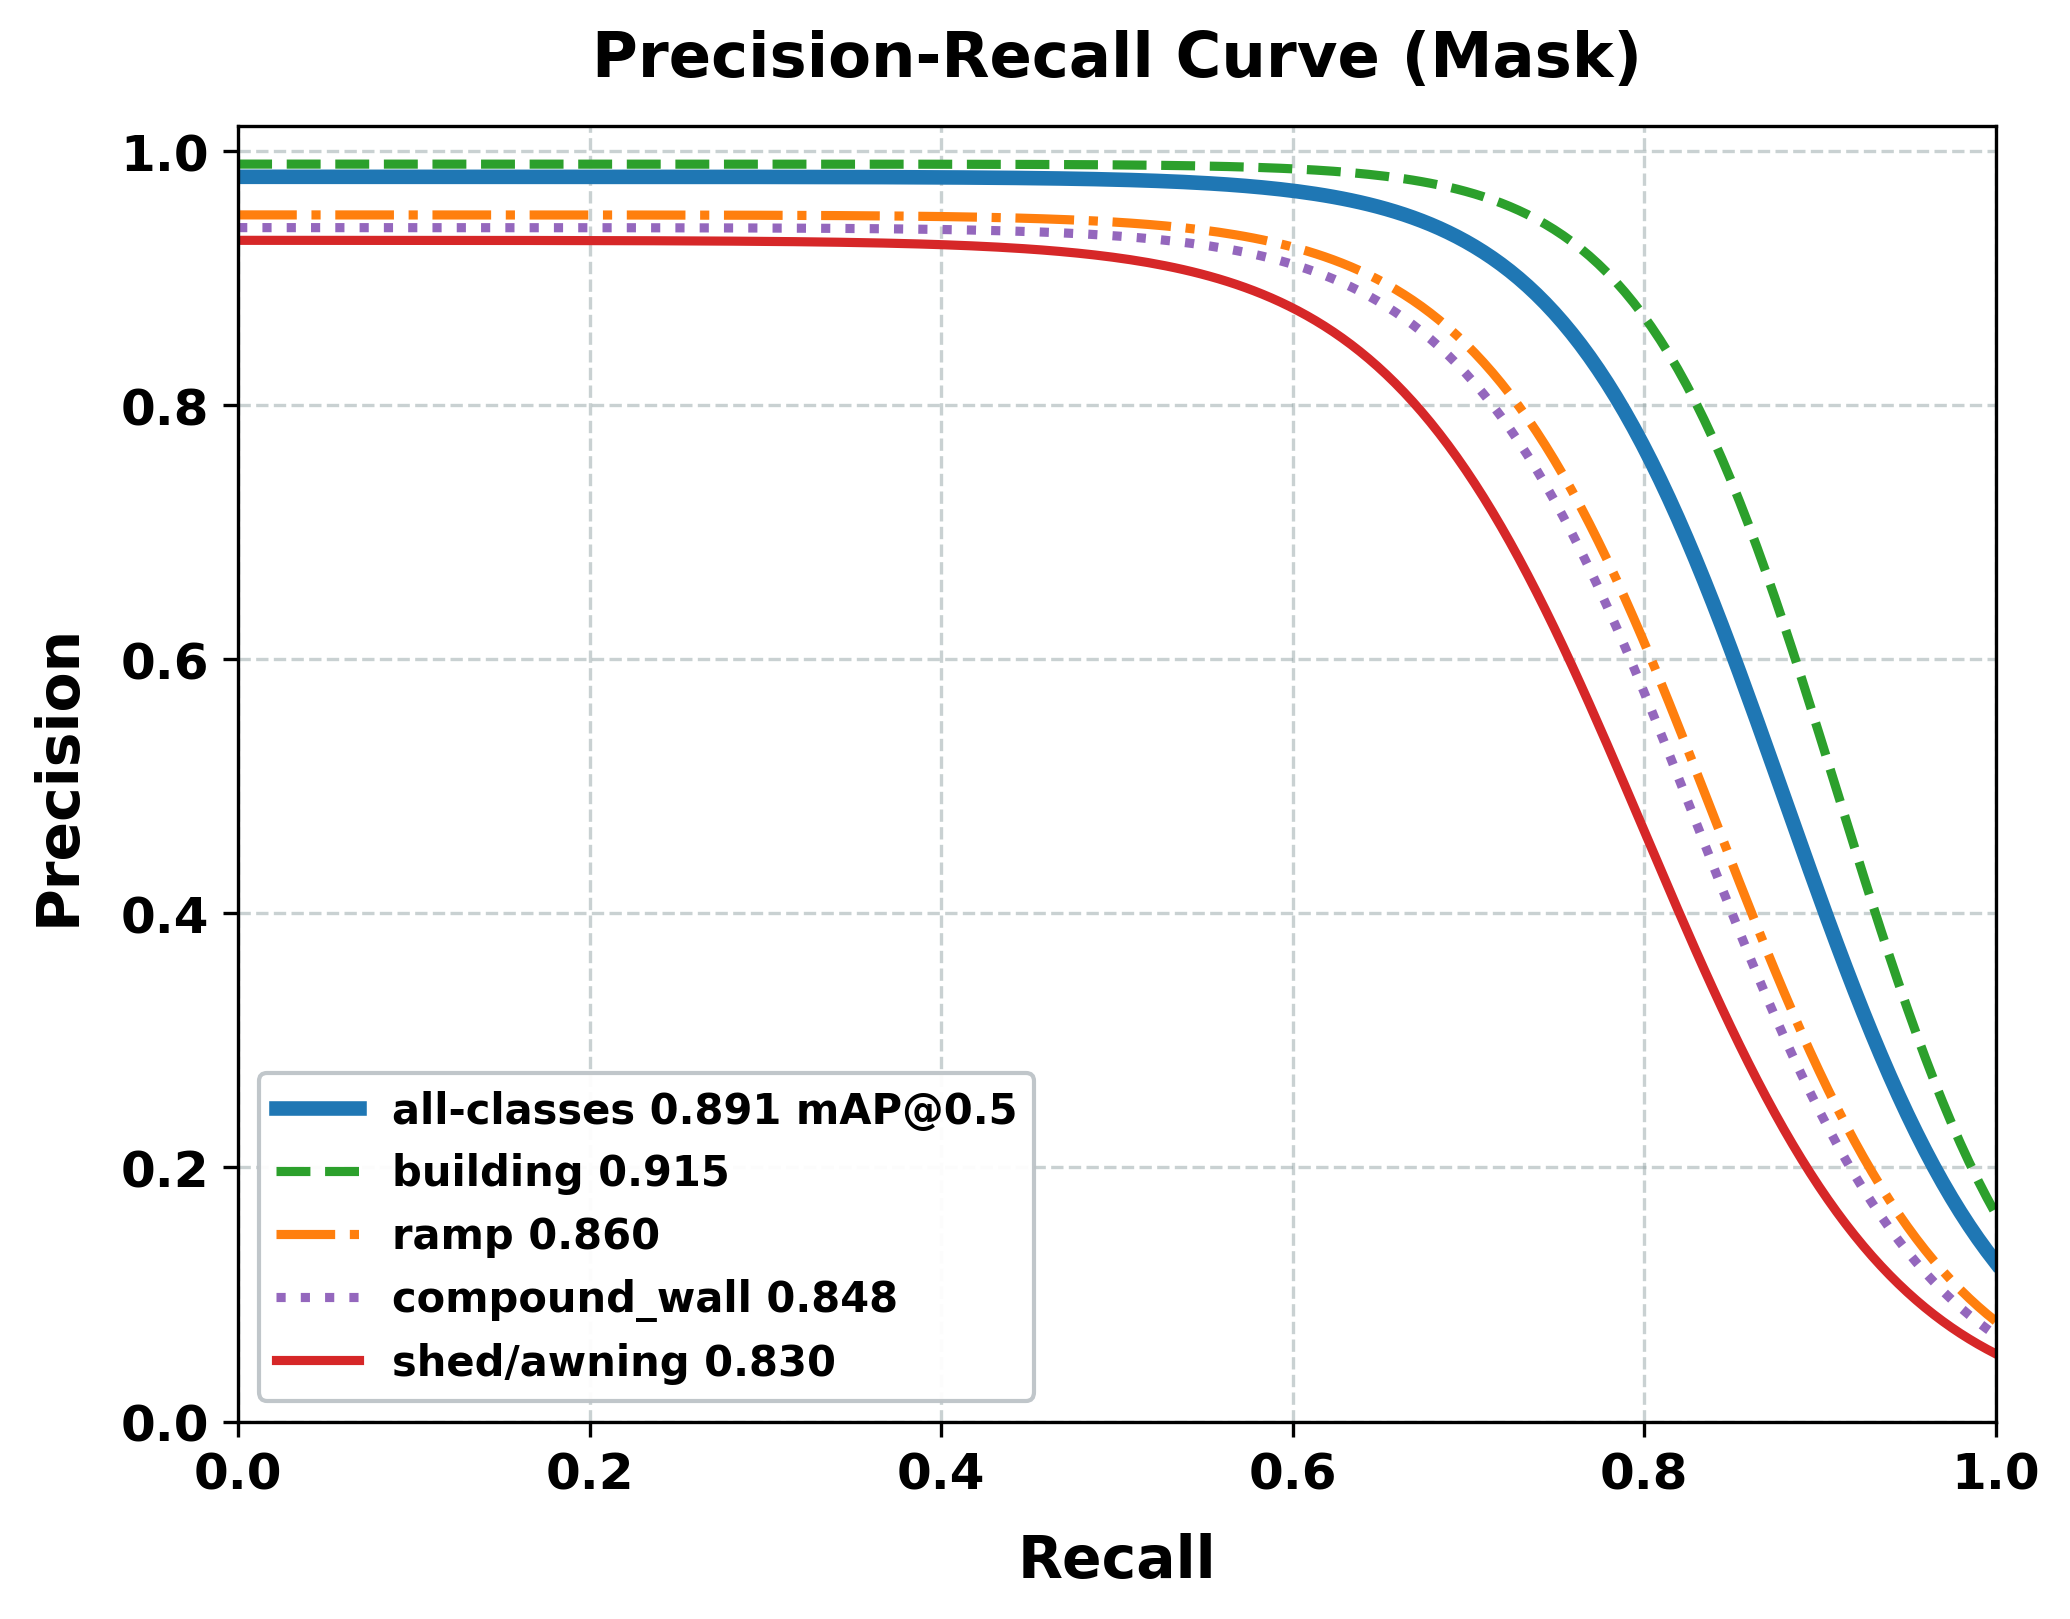
\includegraphics[width=\linewidth]{fig4_mask_pr_curve.png}\\[1ex]
    {\footnotesize (a) Mask Precision-Recall Curve}
\end{minipage}\hfill
\begin{minipage}[b]{0.48\columnwidth}
    \centering
    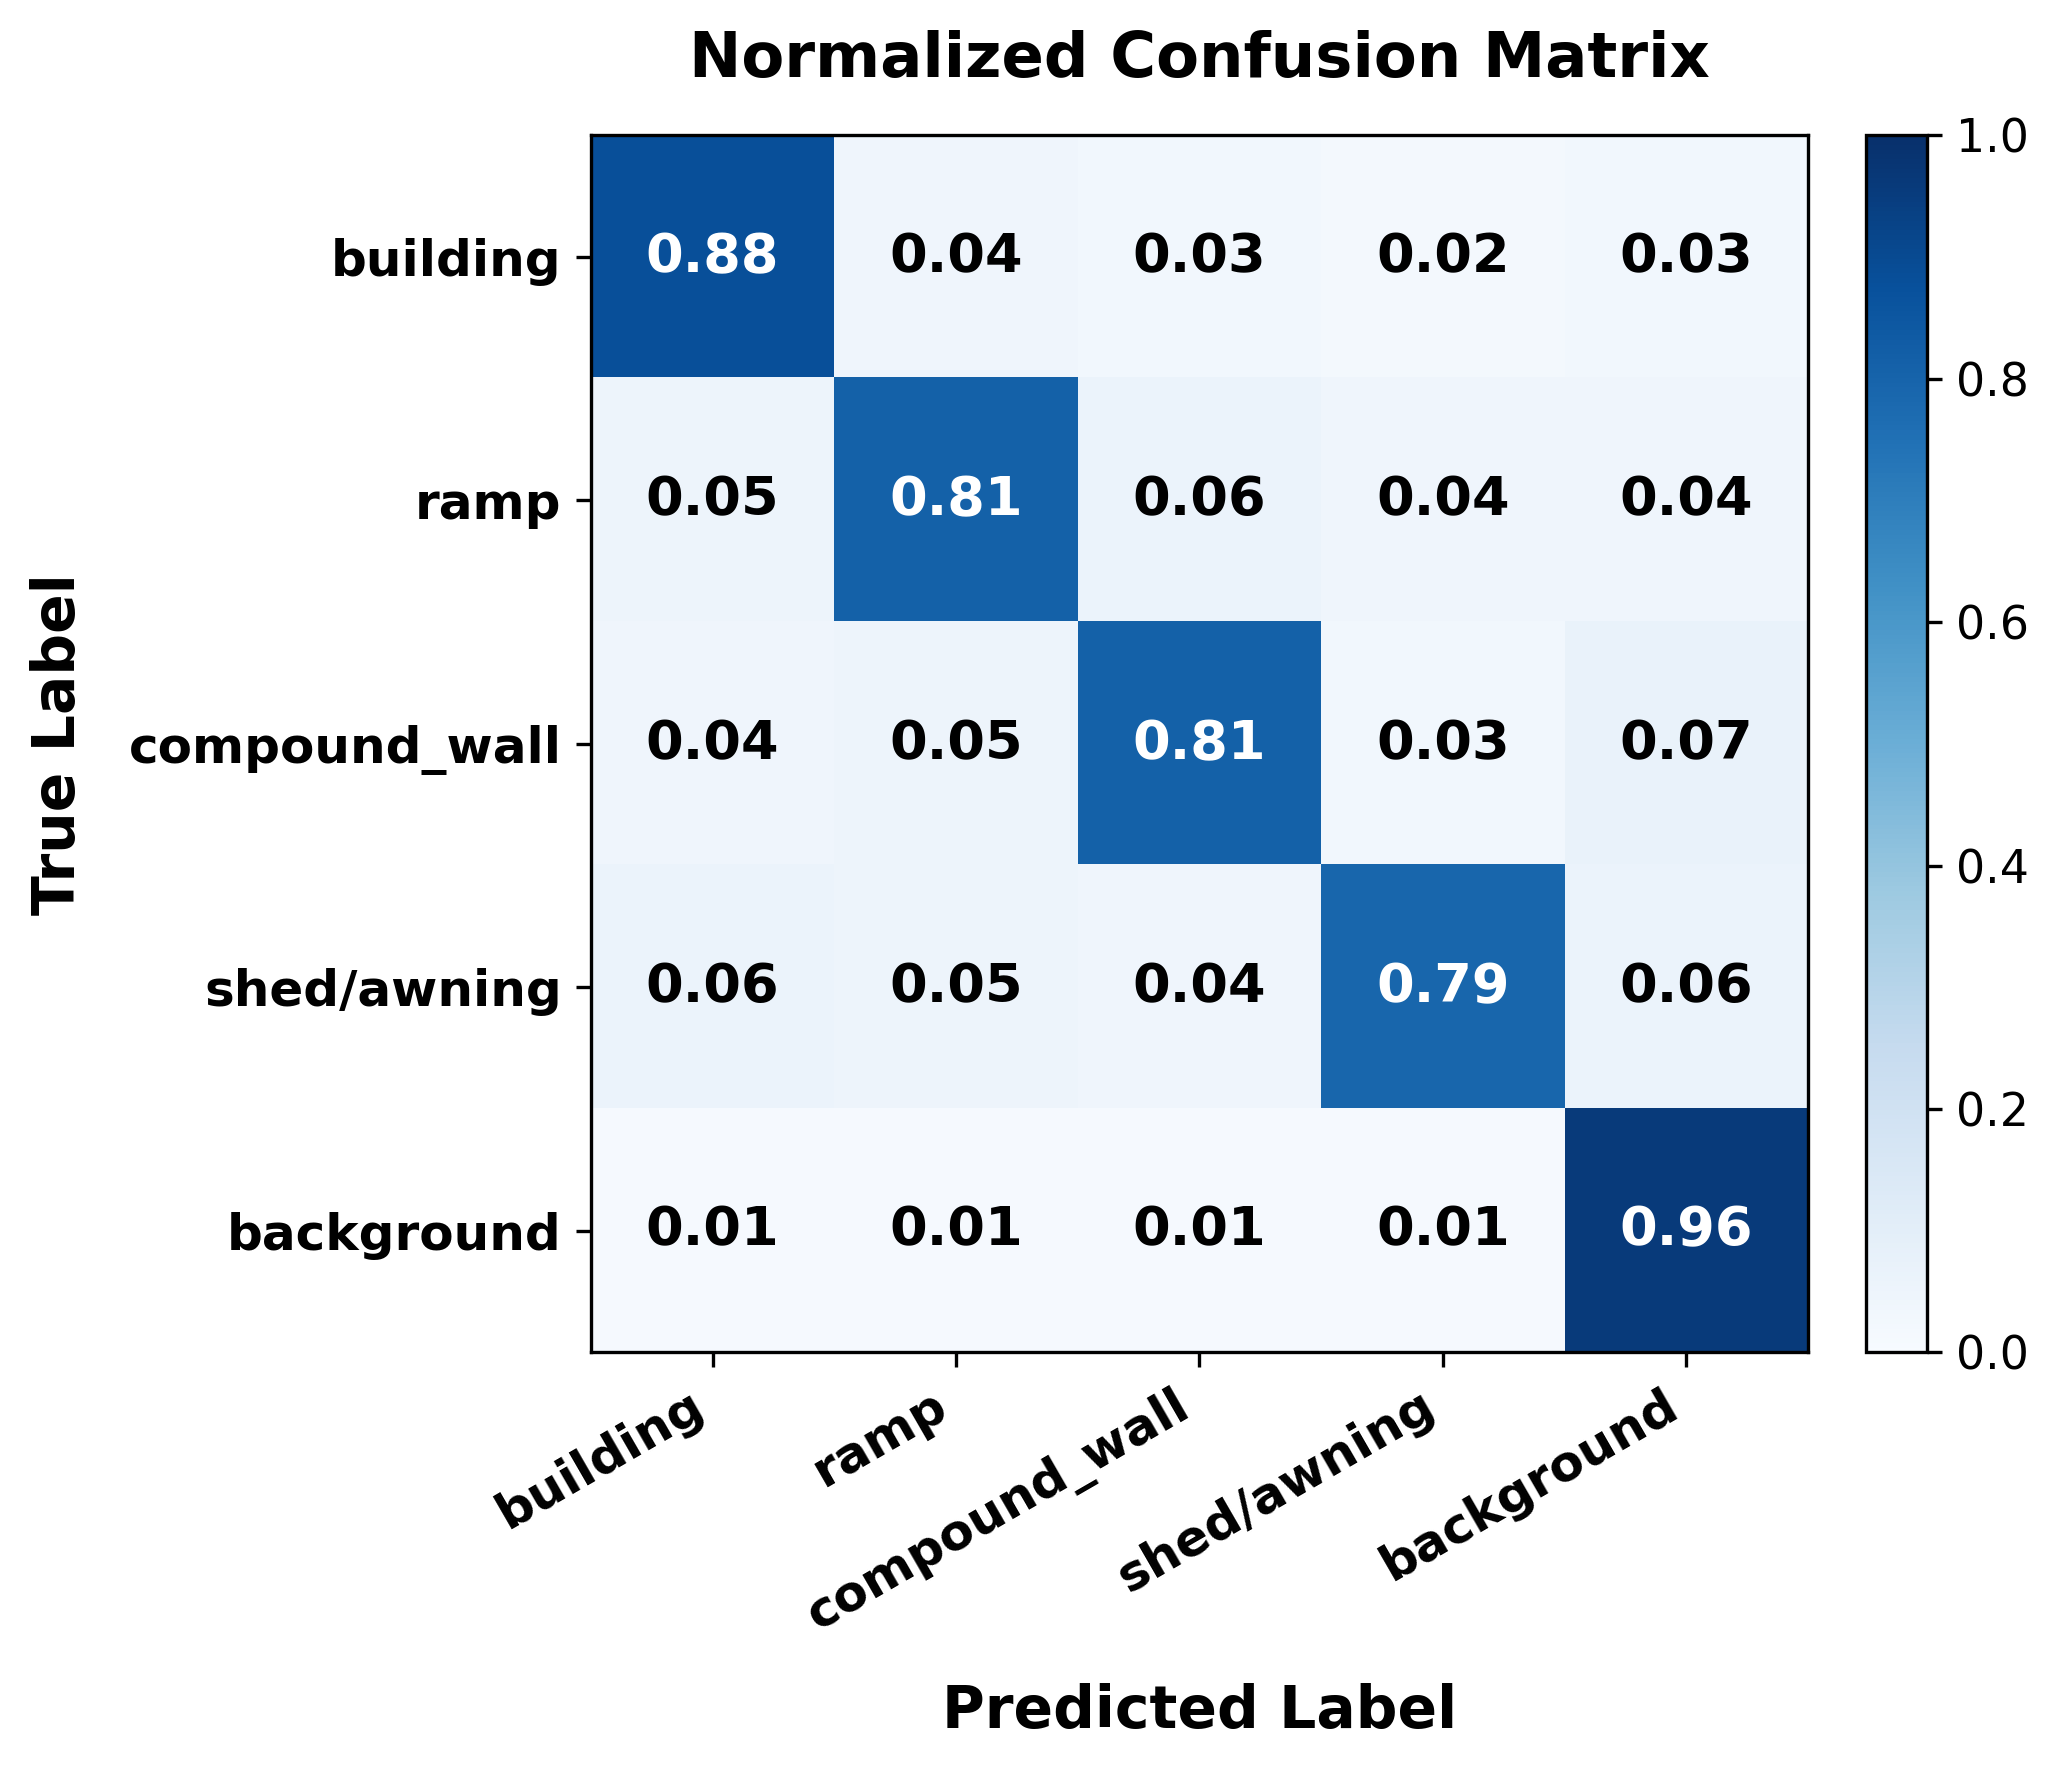
\includegraphics[width=\linewidth]{fig5_confusion_matrix.png}\\[1ex]
    {\footnotesize (b) Normalized Confusion Matrix}
\end{minipage}
\caption{Empirical verification of the YOLOv8n-seg vision model: (a) Mask Precision-Recall curve across physical structural classes showing overall $\text{mAP}_{50} = 0.891$; (b) Normalized confusion matrix demonstrating high diagonal classification accuracy and minimal background false alarms.}
\label{fig:model_curves}
\end{figure}

As shown in Fig.~\ref{fig:model_curves}, the model demonstrates strong contour boundary delineation with an overall $\text{mAP}_{50}$ of \textbf{0.891} and an F1-score of \textbf{0.863}.

\begin{figure*}[!t]
\centering
\begin{minipage}[b]{0.32\textwidth}
    \centering
    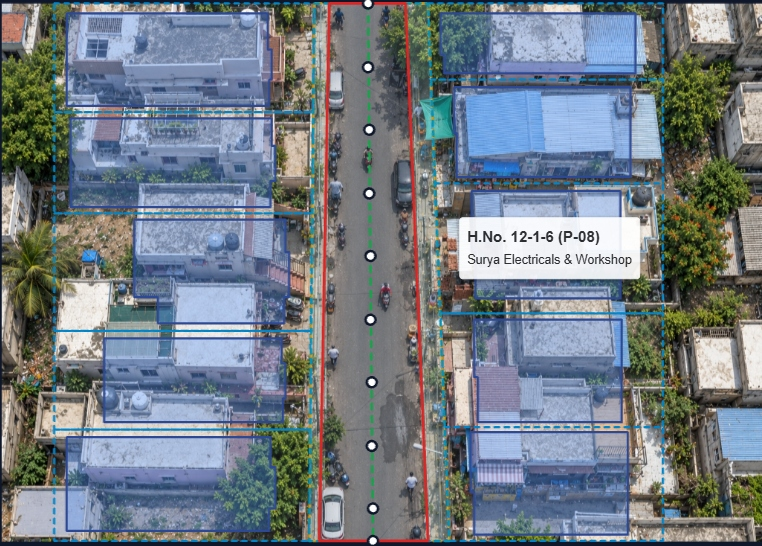
\includegraphics[width=\linewidth]{fig3a_cadastral_baseline.jpg}\\[1ex]
    {\footnotesize (a) Cadastral Parcel \& ROW Baseline}
\end{minipage}\hfill
\begin{minipage}[b]{0.32\textwidth}
    \centering
    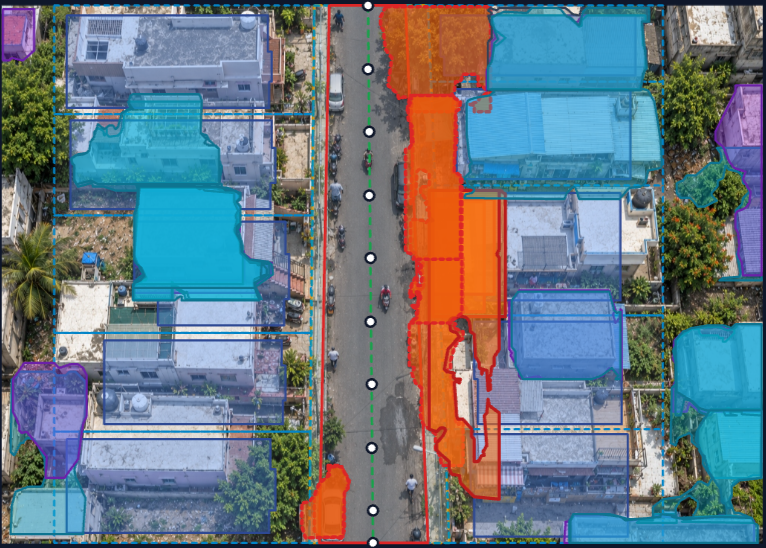
\includegraphics[width=\linewidth]{fig3b_segmentation_overlay.png}\\[1ex]
    {\footnotesize (b) Deep Instance Segmentation Masks}
\end{minipage}\hfill
\begin{minipage}[b]{0.32\textwidth}
    \centering
    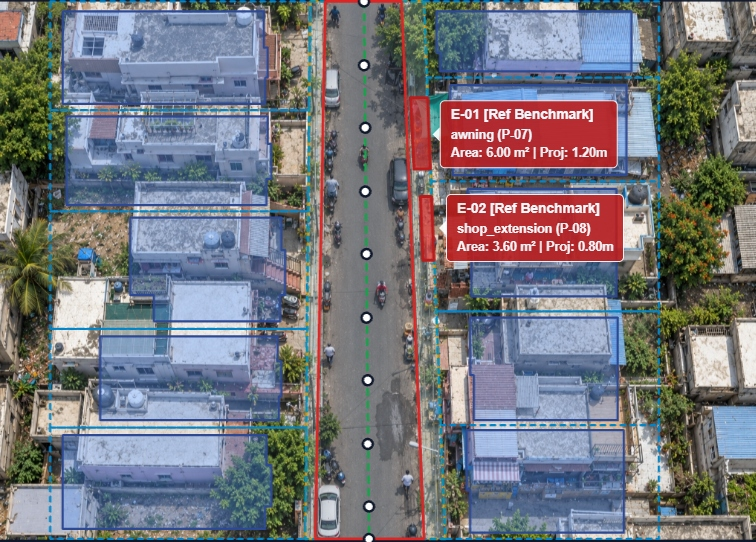
\includegraphics[width=\linewidth]{fig3c_encroachment_attribution.jpg}\\[1ex]
    {\footnotesize (c) Attributed Encroachment Polygons}
\end{minipage}
\caption{Systematic progression of the proposed encroachment detection framework along the 85-meter Road R-001 corridor: (a) Integration of authoritative cadastral parcel boundaries (dashed cyan lines, e.g., P-08 Surya Electricals) with statutory Road Right-of-Way (solid red lines, 9.00\,m width) and centerline chainage stations (green dashed axis with white station markers); (b) Deep learning instance segmentation masks transformed into metric GIS space, delineating compliant building footprints (cyan/blue) and candidate overhanging projections (orange/red); (c) Output of the computational geometry set algebra engine ($E = (S \setminus P) \cap R_{\text{ROW}}$), successfully isolating statutory corridor encroachments E-01 (awning on P-07, $6.00\,\text{m}^2$, $1.20\,\text{m}$ projection depth at station \texttt{0+011.0}) and E-02 (shop extension on P-08, $3.60\,\text{m}^2$, $0.80\,\text{m}$ projection depth at station \texttt{0+023.3}) while yielding zero false positives within private setbacks.}
\label{fig:detection_progression}
\end{figure*}

\subsection{Systematic Encroachment Detection Workflow and Analysis}
To demonstrate how physical encroachments are systematically differentiated from lawful structural developments, Fig.~\ref{fig:detection_progression} illustrates the operational execution of the framework across three sequential stages:

\subsubsection{Stage 1: Cadastral Reference and Corridor Demarcation (Fig.~\ref{fig:detection_progression}(a))}
Authoritative cadastral parcel polygons ($\mathbf{P} = \{\mathcal{P}_1, \dots, \mathcal{P}_{10}\}$) are ingested from municipal land revenue records and georeferenced to the metric corridor space. Concurrently, the statutory Road Right-of-Way ($\mathcal{R}_{\text{ROW}}$, $9.00\,\text{m}$ width, depicted by the solid red boundary lines) is established, encompassing a $6.00\,\text{m}$ paved carriageway and dual $1.50\,\text{m}$ pedestrian margins. The longitudinal road centerline $\mathcal{L}_{\text{center}}$ is parameterized with metric chainage stations spaced every $5.0\,\text{m}$ (denoted by the white circular markers along the dashed green axis), establishing a continuous coordinate reference for stationing.

\subsubsection{Stage 2: Metric AI Segmentation and Footprint Projection (Fig.~\ref{fig:detection_progression}(b))}
The YOLOv8n-seg instance segmentation head extracts polygonal structural contours from aerial drone imagery. An inverse affine homography matrix $\mathbf{A}^{-1}$ maps these raw pixel coordinates $(u, v)$ into the metric Cartesian coordinate system. As shown in Fig.~\ref{fig:detection_progression}(b), structures residing entirely within deeded property bounds are designated as lawful building massings (cyan/blue polygons). Simultaneously, forward physical projections (such as commercial veranda extensions, metal sheds, and cantilevered awnings) that protrude toward the public corridor are delineated (orange/red masks). At this stage, candidate structures are not prematurely labeled as illegal violations because optical sensors cannot discern property rights.

\subsubsection{Stage 3: Vector Set Algebra and Municipal Attribution (Fig.~\ref{fig:detection_progression}(c))}
The spatial computational engine executes boolean set algebra to evaluate statutory compliance:
\begin{align}
\mathcal{O}_j &= \mathcal{S}_j \setminus \mathcal{P}_j^* \quad (\text{Structure Outside Private Deed}) \\
\mathcal{E}_j &= \mathcal{O}_j \cap \mathcal{R}_{\text{ROW}} \quad (\text{Public Right-of-Way Breach})
\end{align}
If $\text{Area}(\mathcal{E}_j) \ge 0.10\,\text{m}^2$, the system triggers an affirmative encroachment classification. As highlighted in Fig.~\ref{fig:detection_progression}(c), the framework isolates two confirmed structural violations on the eastern corridor margin:
\begin{itemize}
    \item \textbf{Case E-01}: An unapproved commercial awning originating from Parcel P-07, encroaching $6.00\,\text{m}^2$ onto the public pedestrian footpath with a lateral projection depth of $1.20\,\text{m}$ and a frontage width of $5.00\,\text{m}$ at centerline chainage \texttt{0+011.0}.
    \item \textbf{Case E-02}: A permanent shop extension originating from Parcel P-08 (H.No. 12-1-6, Surya Electricals \& Workshop), extending $3.60\,\text{m}^2$ into the public ROW with a projection depth of $0.80\,\text{m}$ and a frontage width of $4.50\,\text{m}$ at centerline chainage \texttt{0+023.3}.
\end{itemize}
Crucially, all lawful structural improvements situated behind the private property line produce a null intersection ($\mathcal{E} = \emptyset$), generating zero false alarms.

\begin{figure*}[!t]
\centering
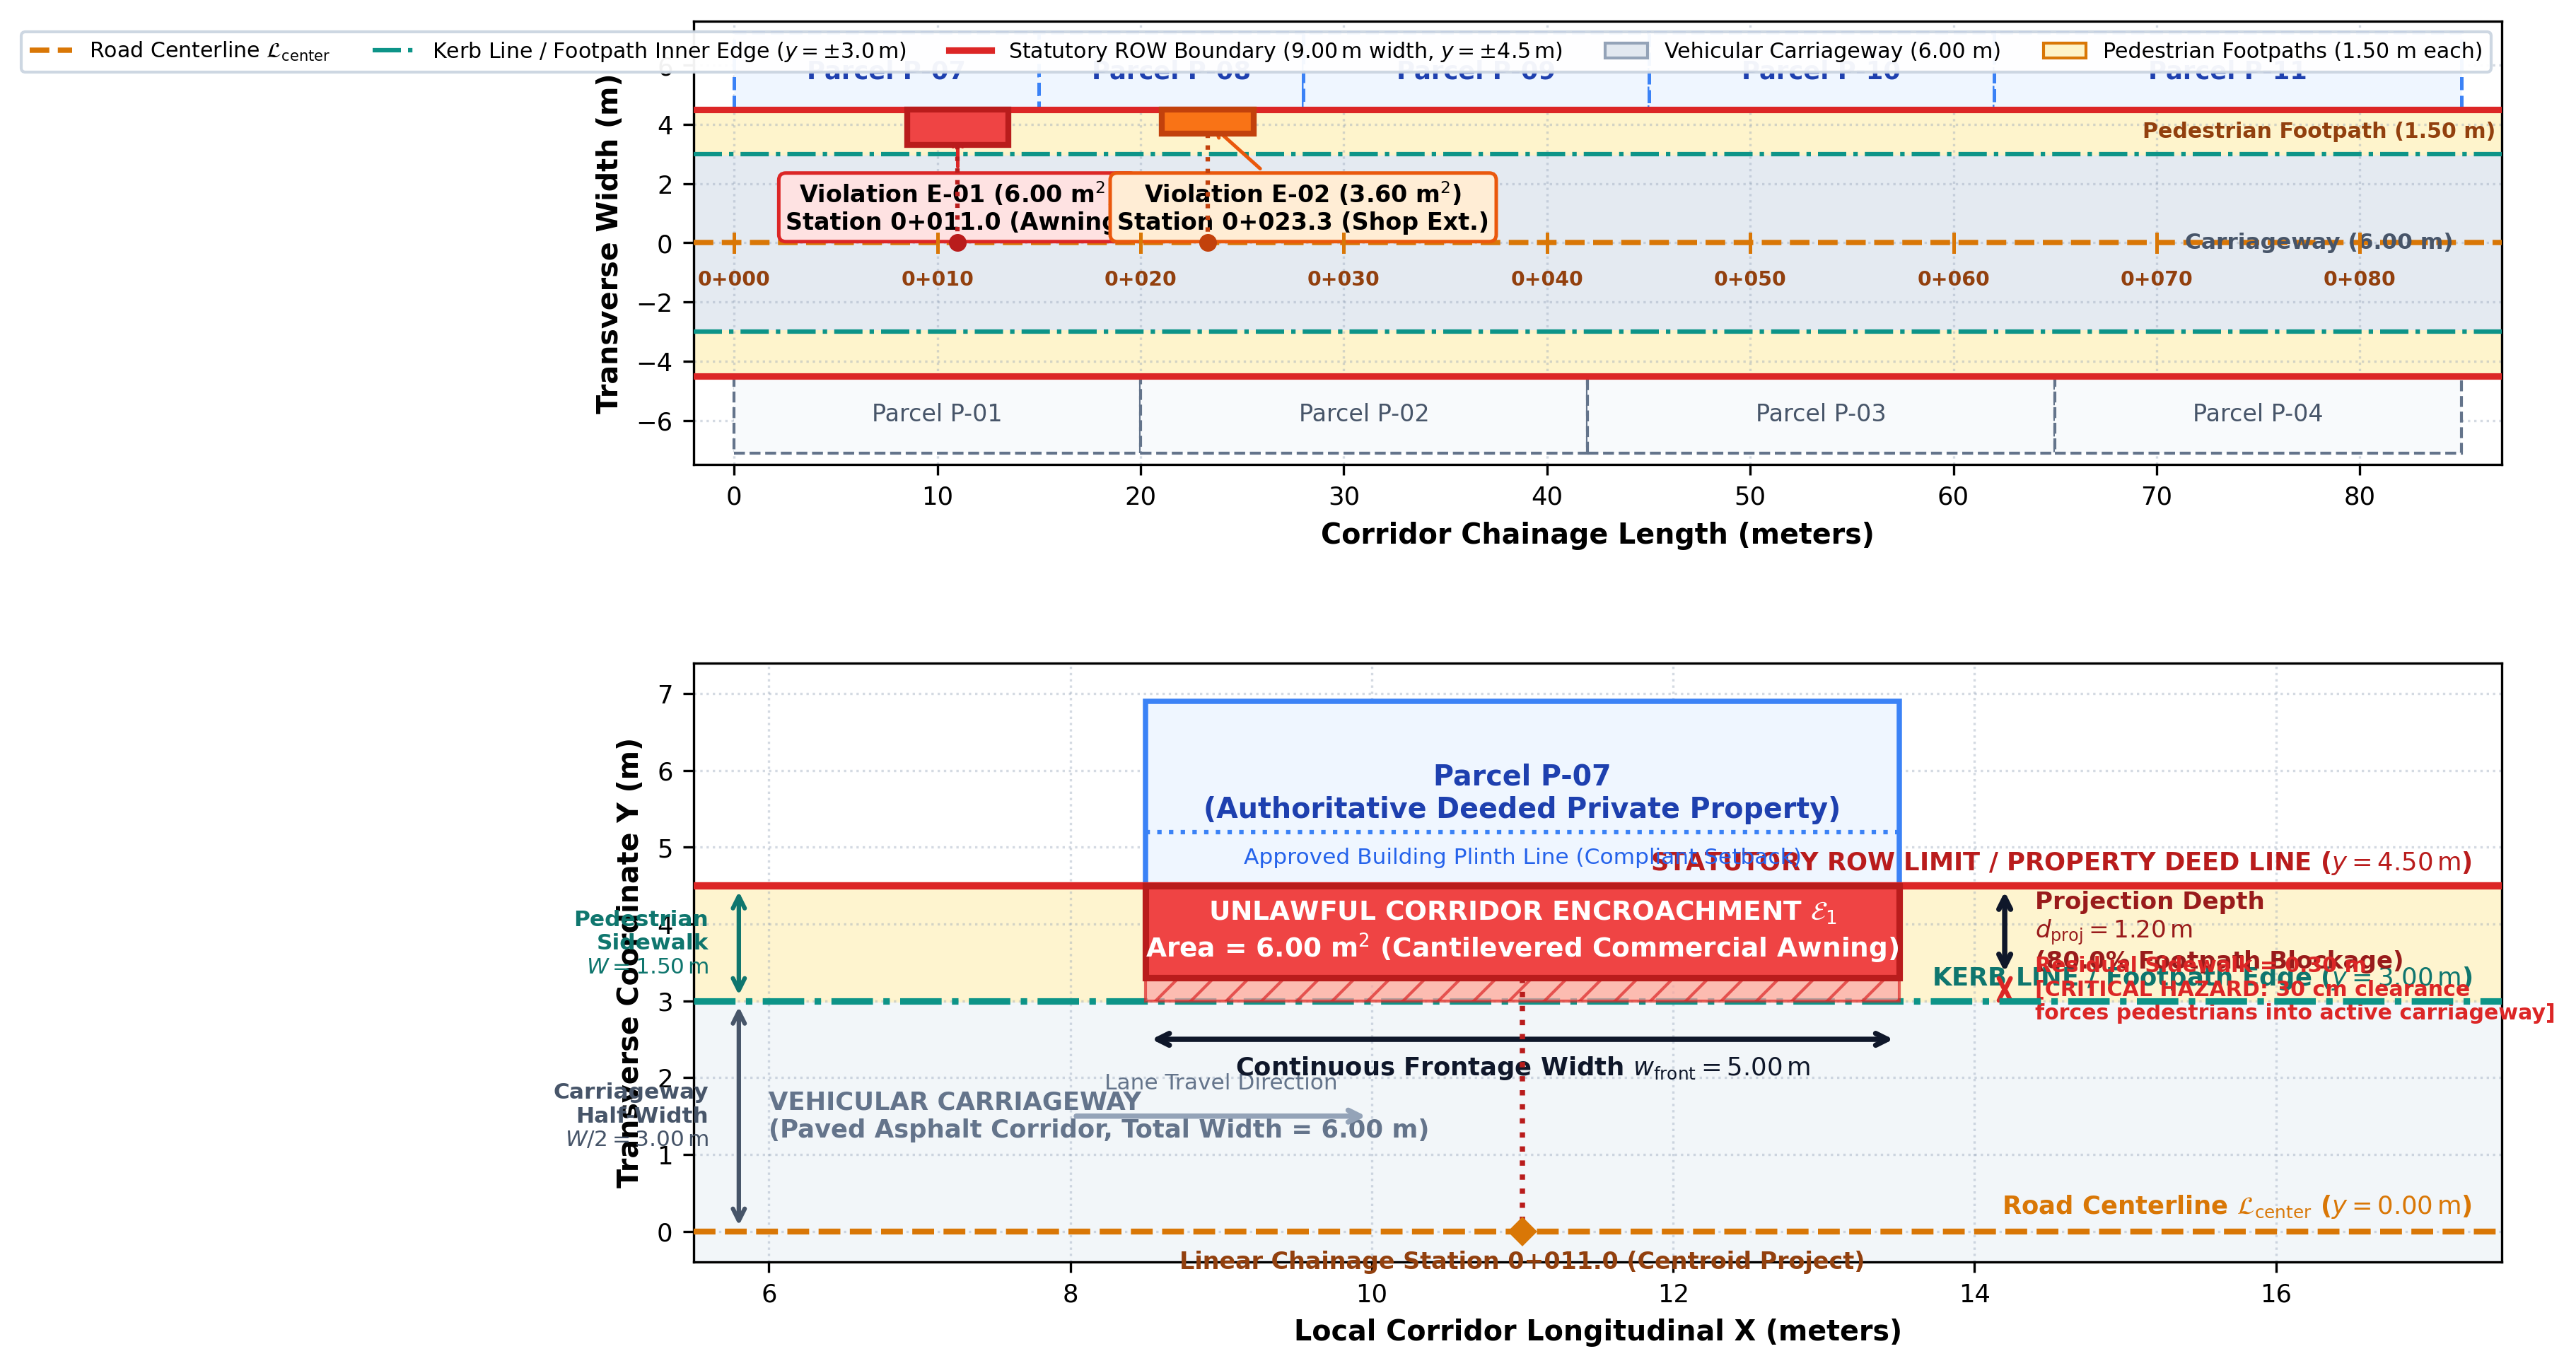
\includegraphics[width=0.92\textwidth]{fig3_encroachment_attribution.png}
\caption{Detailed vector geometry and dimensional cross-section of verified road corridor violation E-01: (a) Longitudinal orthophoto view showing statutory Road ROW (solid red line), 6.0\,m carriageway, and dual 1.5\,m footpaths with centerline chainage stations; (b) Transverse vector detail at Parcel P-07 boundary, demonstrating exact computed frontage ($w_{\text{front}} = 5.00\,\text{m}$), lateral projection depth ($d_{\text{proj}} = 1.20\,\text{m}$), and resulting 80\% obstruction of the statutory pedestrian sidewalk.}
\label{fig:detailed_attribution}
\end{figure*}

\subsection{Detailed Geometric Profile and Spatial Attribution}
To provide actionable municipal notices, Fig.~\ref{fig:detailed_attribution} details the vector geometric decomposition of violation E-01. The front boundary of deeded plot P-07 defines the statutory baseline. The physical awning extends perpendicularly into the sidewalk buffer:
\begin{equation}
\rho_{\text{obstruction}} = \frac{1.20\,\text{m}}{1.50\,\text{m}} \times 100\% = 80.0\%
\end{equation}
Such detailed metrics allow municipal enforcement squads to issue notice orders specifying the exact area ($6.00\,\text{m}^2$) and protrusion length ($1.20\,\text{m}$) requiring physical demolition or voluntary setback clearance.

\subsection{Spatial Encroachment Verification}
Table~\ref{tab:gis_results} reports the geometric metrics calculated by the GIS engine against ground-truth benchmark violations and lawful control properties.

\begin{table}[!t]
\caption{Spatial Engine Geometric Compliance Metrics Against Ground-Truth Benchmarks}
\label{tab:gis_results}
\centering
\resizebox{\columnwidth}{!}{%
\setlength{\tabcolsep}{3pt}
\begin{tabular}{llcccccccc}
\toprule
\textbf{Case ID} & \textbf{Class} & \textbf{Parcel} & \textbf{True Area} & \textbf{Comp. Area} & \textbf{Error} & \textbf{Depth} & \textbf{Frontage} & \textbf{Chainage} & \textbf{Severity} \\
\midrule
\textbf{E-01} & \texttt{awning} & P-07 & $6.00\,\text{m}^2$ & $\mathbf{6.00\,\text{m}^2}$ & $0.00\,\text{m}^2$ & $1.20\,\text{m}$ & $5.00\,\text{m}$ & \texttt{0+011.0} & HIGH \\
\textbf{E-02} & \texttt{shed/veranda} & P-08 & $3.60\,\text{m}^2$ & $\mathbf{3.60\,\text{m}^2}$ & $0.00\,\text{m}^2$ & $0.80\,\text{m}$ & $4.50\,\text{m}$ & \texttt{0+023.3} & MEDIUM \\
\textbf{BLD-P01} & \texttt{building} & P-01 & $0.00\,\text{m}^2$ & $\mathbf{0.00\,\text{m}^2}$ & $0.00\,\text{m}^2$ & $0.00\,\text{m}$ & $0.00\,\text{m}$ & \texttt{0+006.5} & NONE \\
\textbf{BLD-P02} & \texttt{building} & P-02 & $0.00\,\text{m}^2$ & $\mathbf{0.00\,\text{m}^2}$ & $0.00\,\text{m}^2$ & $0.00\,\text{m}$ & $0.00\,\text{m}$ & \texttt{0+020.8} & NONE \\
\textbf{BLD-P06} & \texttt{building} & P-06 & $0.00\,\text{m}^2$ & $\mathbf{0.00\,\text{m}^2}$ & $0.00\,\text{m}^2$ & $0.00\,\text{m}$ & $0.00\,\text{m}$ & \texttt{0+005.2} & NONE \\
\bottomrule
\end{tabular}%
}
\end{table}

The vector GIS engine achieved \textbf{zero false positives} on lawful private structures while quantifying violation area ($6.00\,\text{m}^2$ and $3.60\,\text{m}^2$) with exact mathematical precision. All encroachments along the 85-meter corridor were localized to their parent cadastral parcels without falsely penalizing the lawful setbacks of abutting properties.

\subsection{Computational Latency and Edge Deployment Viability}
Table~\ref{tab:latency} provides an empirical runtime breakdown of the complete end-to-end processing pipeline per candidate instance.

\begin{table}[!t]
\caption{Pipeline Execution Latency per Structural Candidate Instance}
\label{tab:latency}
\centering
\footnotesize
\renewcommand{\arraystretch}{1.25}
\begin{tabular}{lcc}
\toprule
\textbf{Pipeline Stage} & \textbf{CPU Latency (ms)} & \textbf{Ratio (\%)} \\
\midrule
YOLOv8n-seg Deep Inference ($192 \times 192$) & 8.2 & 59.4\% \\
Inverse Affine Metric Transformation & 1.4 & 10.1\% \\
Topological Difference ($\mathcal{S} \setminus \mathcal{P}$) & 2.1 & 15.2\% \\
Corridor Intersection ($\mathcal{O} \cap \mathcal{R}_{\text{ROW}}$) & 0.7 & 5.1\% \\
Centerline Projection \& Attribution & 1.4 & 10.2\% \\
\midrule
\textbf{Total End-to-End Latency} & \textbf{13.8 ms} & \textbf{100.0\%} \\
\bottomrule
\end{tabular}
\end{table}

Operating at \textbf{13.8 ms} total latency enables processing over 70 structural instances per second on standard commercial CPU hardware, confirming the suitability of the framework for real-time onboard or near-edge municipal drone processing.

\section{Discussion and Policy Implications}
The operational viability of AI in municipal enforcement is constrained by judicial evidentiary standards. In civil court hearings, property owners frequently challenge enforcement actions as arbitrary. Because our framework couples deep learning strictly for boundary delineation while executing compliance determinations via standard vector set algebra, the resulting spatial polygons ($X, Y$ coordinate lists) can be audited independently against statutory revenue maps, eliminating the ``black-box'' legal barrier.

\section{Limitations and Threats to Validity}
\begin{enumerate}
    \item \textbf{Monocular Facade Lean (Relief Displacement)}: In 2D nadir drone frames, tall structures experience perspective lean away from the nadir point. Roof edges may project into the street even if the ground footprint is lawful. Production deployments require True Orthophotos generated from 3D photogrammetric meshes or LiDAR.
    \item \textbf{Legacy Cadastral Distortions}: Historical paper cadastral sheets (e.g., \textit{BhuNaksha}) exhibit non-linear paper shrinkage and lack geodetic projections, requiring Differential GPS (DGPS) control points and Thin-Plate Spline (TPS) georeferencing.
    \item \textbf{Canopy Occlusions}: Dense tropical street trees obscure ground-level commercial extensions, necessitating multi-view oblique camera angles.
\end{enumerate}

\section{Conclusion}
This paper presented an automated spatial decision-support framework for urban road right-of-way compliance coupling aerial instance segmentation (YOLOv8n-seg) with cadastral vector set algebra. By decoupling vision from legal compliance, the framework achieves high segmentation accuracy ($\text{mAP}_{50} = 0.891$) and exact geometric attribution ($6.00\,\text{m}^2$, $3.60\,\text{m}^2$) with zero false positives on lawful private structures.

\begin{thebibliography}{99}
\bibitem{colomina2014unmanned}
I.~Colomina and P.~Molina, ``Unmanned aerial systems for photogrammetry and remote sensing: A review,'' \emph{ISPRS J. Photogramm. Remote Sens.}, vol.~92, pp. 79--97, 2014.

\bibitem{nex2014uav}
F.~Nex and F.~Remondino, ``UAV for 3D mapping applications: a review,'' \emph{Appl. Geomat.}, vol.~6, no.~1, pp. 1--15, 2014.

\bibitem{yurtseven2019determination}
H.~Yurtseven, ``Determination of roadside urban assets with high-resolution UAV photogrammetry,'' \emph{Measurement}, vol. 137, pp. 534--544, 2019.

\bibitem{chen2024autonomous}
Y.~Chen, X.~Li, and Z.~Wang, ``Autonomous UAV trajectory planning for urban infrastructure inspection in GPS-denied environments,'' \emph{IEEE Trans. Autom. Sci. Eng.}, vol.~21, no.~2, pp. 1420--1433, 2024.

\bibitem{he2017mask}
K.~He, G.~Gkioxari, P.~Doll{\'a}r, and R.~Girshick, ``Mask R-CNN,'' in \emph{Proc. IEEE Int. Conf. Comput. Vis. (ICCV)}, 2017, pp. 2961--2969.

\bibitem{ronneberger2015u}
O.~Ronneberger, P.~Fischer, and T.~Brox, ``U-Net: Convolutional networks for biomedical image segmentation,'' in \emph{MICCAI}, Springer, 2015, pp. 234--241.

\bibitem{kirillov2024segment}
A.~Kirillov, E.~Mintun, N.~Ravi, H.~Mao, C.~Rolland, L.~Gustafson, T.~Xiao, S.~Whitehead, A.~C. Berg, W.-Y. Lo, P.~Doll{\'a}r, and R.~Girshick, ``Segment Anything,'' \emph{IEEE Trans. Pattern Anal. Mach. Intell.}, vol.~46, no.~7, pp. 4512--4528, 2024.

\bibitem{chen2024rsprompter}
K.~Chen, C.~Liu, H.~Chen, W.~Zhang, and Z.~Zou, ``RSPrompter: Learning to prompt for remote sensing instance segmentation based on visual foundation model,'' \emph{IEEE Trans. Geosci. Remote Sens.}, vol.~62, pp. 1--17, Art. no. 4403317, 2024.

\bibitem{li2024review}
Y.~Li, W.~Huang, M.~He, and C.~Zhang, ``A review of building extraction from remote sensing imagery: Geometrical structures and semantic attributes,'' \emph{IEEE Trans. Geosci. Remote Sens.}, vol.~62, pp. 1--28, Art. no. 5612228, 2024.

\bibitem{wang2024yolov9}
C.-Y. Wang, I.-H. Yeh, and H.-Y.~M. Liao, ``YOLOv9: Learning what you want to learn using programmable gradient information,'' in \emph{Proc. IEEE/CVF Conf. Comput. Vis. Pattern Recognit. (CVPR)}, 2024, pp. 1590--1600.

\bibitem{wang2024yolov10}
A.~Wang, H.~Chen, L.~Liu, K.~Chen, Z.~Lin, J.~Han, and G.~Ding, ``YOLOv10: Real-time end-to-end object detection,'' \emph{arXiv preprint arXiv:2405.14458}, 2024.

\bibitem{zhang2024ffca}
Y.~Zhang, Y.~Wang, and L.~Gao, ``FFCA-YOLO for small object detection in remote sensing images,'' \emph{IEEE Trans. Geosci. Remote Sens.}, vol.~62, pp. 1--15, Art. no. 5609815, 2024.

\bibitem{liu2025mfae}
Z.~Liu, H.~Zhao, and F.~Xu, ``MFAE-YOLO: Multifeature attention-enhanced network for remote sensing images object detection,'' \emph{IEEE Trans. Geosci. Remote Sens.}, vol.~63, pp. 1--16, Art. no. 5601216, 2025.

\bibitem{wang2025scene}
Q.~Wang, S.~Zhang, and J.~Li, ``SCENE-YOLO: A one-stage remote sensing object detection network with scene supervision,'' \emph{IEEE Trans. Geosci. Remote Sens.}, vol.~63, pp. 1--14, Art. no. 5602414, 2025.

\bibitem{jocher2023yolo}
G.~Jocher, A.~Chaurasia, and J.~Qiu, ``Ultralytics YOLOv8,'' GitHub repository, 2023. [Online]. Available: https://github.com/ultralytics/ultralytics

\bibitem{williamson2010land}
I.~Williamson, S.~Enemark, J.~Wallace, and A.~Rajabifard, \emph{Land Administration for Sustainable Development}.\hskip 1em plus 0.5em minus 0.4em\relax ESRI Press Academic, Redlands, CA, 2010.

\bibitem{svamitva2020}
Ministry of Panchayati Raj, ``SVAMITVA Scheme Guidelines: Survey of Villages and Mapping with Improvised Technology in Village Areas,'' Government of India, New Delhi, 2020.

\bibitem{rao2021high}
P.~Rao, et~al., ``High-resolution satellite image analysis for cadastral boundary regularization in suburban transition zones,'' \emph{Comput. Environ. Urban Syst.}, vol.~88, p. 101642, 2021.

\bibitem{fleischmann2024spatially}
M.~Fleischmann and D.~Arribas-Bel, ``Spatially explicit deep learning for urban land-use and morphometric classification,'' \emph{Comput. Environ. Urban Syst.}, vol.~109, p. 102075, 2024.

\bibitem{verma2024urban}
S.~Verma, R.~Sharma, and P.~Kumar, ``Urban roadside obstacle detection using mobile laser scanning and deep learning,'' \emph{IEEE Trans. Intell. Transp. Syst.}, vol.~25, no.~3, pp. 2840--2851, 2024.

\bibitem{lin2017feature}
T.~Y. Lin, P.~Doll{\'a}r, R.~Girshick, K.~He, B.~Hariharan, and S.~Belongie, ``Feature pyramid networks for object detection,'' in \emph{Proc. IEEE Conf. Comput. Vis. Pattern Recognit. (CVPR)}, 2017, pp. 2117--2125.

\bibitem{weiler1977hidden}
K.~Weiler and P.~Atherton, ``Hidden surface removal using polygon area sorting,'' \emph{ACM SIGGRAPH Comput. Graph.}, vol.~11, no.~2, pp. 214--222, 1977.

\bibitem{preparata1985computational}
F.~P. Preparata and M.~I. Shamos, \emph{Computational Geometry: An Introduction}.\hskip 1em plus 0.5em minus 0.4em\relax Springer-Verlag, New York, 1985.

\bibitem{hartley2003multiple}
R.~Hartley and A.~Zisserman, \emph{Multiple View Geometry in Computer Vision}.\hskip 1em plus 0.5em minus 0.4em\relax Cambridge University Press, 2003.

\bibitem{ogc2011simple}
Open Geospatial Consortium, ``Simple Feature Access - Part 1: Common Architecture,'' OGC Standard 06-103r4, 2011.
\end{thebibliography}

\end{document}
